
\hypertarget{ejercicios}{%
\section*{Ejercicios}\label{ejercicios}}
\addcontentsline{toc}{section}{Ejercicios}


\begin{ejercicio}¿Qué resultado producen las siguientes expresiones?

(a)  \pythoninline{True and not False}

(b) \pythoninline{True or not True}

(c) \pythoninline{True or True and False }

(d) \pythoninline{not True or not False }

(e) \pythoninline{True and not 0 }

(f) \pythoninline{52 < 52.3 }

(g) \pythoninline{1 + 52 < 52.3 }

(h) \pythoninline{4 \!= 4.0}

(i) \pythoninline{'melocotón' < 'manzana'}

(j)  \pythoninline{'elefante' > 'Ratón'}
\end{ejercicio}


\respuesta{
a. True
b. True 
c. True 
d. True 
e. True
f. True
g. False
h. False
}

\begin{ejercicio}Escribe una expresión en Python que devuelva True si un entero dado n es mayor a 100 o menor a 0.
\end{ejercicio}
\respuesta{
\pythoninline{(n > 100) or (n < 0)}
}

\begin{ejercicio}Escribe una expresión en Python que devuelva True si un entero dado n es impar y está en el intervalo [2, 16[.
\end{ejercicio}
\respuesta{\pythoninline{(n \% 2 == 0) and (n >=2 and n < 16)}}

\begin{ejercicio}Imagina que a y b son variables booleanas. Escribe expresiones en Python que:

(a) resulta en True si y solo si las dos variables son True

(b) resulta en True si y solo si a es False

(c) resulta en True si y solo si como mínimo una de los variables es True.
\end{ejercicio}
\respuesta{
a. \pythoninline{a and b }

b. \pythoninline{not a }

c. \pythoninline{a or b}
}


\begin{ejercicio}Variables full y empty son variables de tipo booleano. Escribe una expresión en Python que resulta en True cuando como máximo una de los variables es True.
\end{ejercicio}
\respuesta{
\pythoninline{(full or empty) and not (full and empty)}
}

\begin{ejercicio}
Escribe una expresión en Python que devuelva True si una variable \verb|year| de tipo int contiene un entero que representa un año bisiesto.

Un año es bisiesto si es divisible por 4 y no divisible por 100, excepto si es también divisible por 400, en cuyo caso es bisiesto.
\end{ejercicio}



\begin{ejercicio}Escribe un programa que, dado un número devuelve si es par o impar.

Puedes testear tu programa con los siguientes casos de test:\\

\begin{Verbatim}[frame=single, label={\em example test execution of the program}]
>>> %Run 
Enter a number: 4
The number is even
>>> %Run 
Enter a number: 7
The number is uneven
>>> %Run 
Enter a number: 0
The number is even
>>> %Run 
Enter a number: -4
The number is even
>>> %Run 
Enter a number: -101
The number is uneven
\end{Verbatim}
\end{ejercicio}


\begin{ejercicio}En una tienda de electrodomésticos se aplican distintos descuentos en función del total de las compras realizadas:

\begin{itemize}
\item Si total < 500 euro, no se aplica descuento.
\item Si 500 € <= total <= 2000 €, se aplica un descuento del 30%.
\item Si total > 2000 €, entonces se aplica un descuento del 50%.
\end{itemize}


Escribe un programa que, dado un total, devuelva la cantidad a pagar (tras aplicar el descuento correspondiente). Se debe resolver el problema con una única instrucción condicional (anidada). Proporcionar dos soluciones completando la instrucción si la condición es total>=500 o total<=2000.\\

Sol.1:
\begin{python}
total = int(input("Introduce el importe total de las compras: "))
if total >= 500:
...
\end{python}

Sol.2:
\begin{python}
total = int(input("Introduce el importe total de las compras: "))
if total <= 2000:
...
\end{python}
\end{ejercicio}



\begin{ejercicio}Queremos que se encienda una cámara de forma automática si el nivel de luz es inferior a 0.01 lux o si la temperatura está por encima de cero, pero no si ambas condiciones son ciertas. (Debe suponer que la función turn-camera-on ya se ha definido). Tu amiga Anna dice que tiene que ser:



\begin{python}
if ((light<0.01) or (temp>0)) and  not ((light<0.01) and (temp>0)):
	turn_camera_on()
\end{python}

Tu amiga Maria dice que eso también se puede escribir más simple usando:

\begin{python}
if (light<0.01) != (temp>0.0):
	turn_camera_on()
\end{python}

¿tienen razón las dos? ¿por que?
\end{ejercicio}

\respuesta{
Si! Imagina que L es \pythoninline{(light<0.01)} y T es \pythoninline{(temp>0.0)}. Podemos hacer una tabla de verdad:


\begin{tabular}{|l|l|l|l|l}
\hline
L & T & L!=T & L or T and not (L and T)  \\
\hline
True                      & True                      & False                        & False           \\
\hline
True                      & False                     & True                         & True        \\
\hline
False                     & True                      & True                         & True                     \\
\hline
False                     & False                     & False                        & False           \\
\hline
\end{tabular}
}




\begin{ejercicio}Completa la siguiente tabla indicando qué instrucción se realiza en función de los valores de condicion1, condicion2 y condicion3. Indica con un \verb|-| cuando la condición no se evalúa.

\begin{python}
if condicion1:
    if condicion2:
        accion1
    else:
        accion2
else:
    if condicion3:
        accion3
    else:
        accion4
\end{python}


\begin{tabular}{|l|l|l|l|}
\hline
condicion1 & condicion2 & condicion3 & instrucción \\
\hline
\hline
           &            &            &             \\ \hline
           &            &            &        
          \\ \hline
                     &            &            &        
          \\ \hline
\end{tabular}
\end{ejercicio}


\begin{ejercicio}\label{prod_sin_mult}
Implementar un programa que lea dos números enteros y diga si su producto es positivo, negativo, o cero \textbf{sin} llegar a realizar dicho producto. \\

Ejecuta los siguientes ejemplos para probar que tu programa da las mismas salidas. Estos ejemplos ejecutan las siguientes combinaciones: 
primer numero es 0, 
segundo numero es 0, 
ambos números son 0, 
ambos números son positivos, 
ambos números son negativos, 
primer numero es negativo y segundo es positivo, 
y primer numero es positivo y segundo es negativo.\\



\begin{Verbatim}[frame=single, label={\em ejemplos y posibles tests de ejecución}]
>>> %Run
  Introduce el primer numero entero: 0
  Introduce el segundo numero entero: -1
  El producto es cero
>>> %Run 
  Introduce el primer numero entero: 5
  Introduce el segundo numero entero: 0
  El producto es cero
>>> %Run 
  Introduce el primer numero entero: 0
  Introduce el segundo numero entero: 0
  El producto es cero
>>> %Run
  Introduce el primer numero entero: 2
  Introduce el segundo numero entero: 7
  El producto es positivo
>>> %Run 
  Introduce el primer numero entero: -4
  Introduce el segundo numero entero: -7
  El producto es positivo
>>> %Run 
  Introduce el primer numero entero: -8
  Introduce el segundo numero entero: 3
  El producto es negativo
>>> %Run 
  Introduce el primer numero entero: 10
  Introduce el segundo numero entero: -6
  El producto es negativo
\end{Verbatim}
\end{ejercicio}



\begin{ejercicio}\label{dados_rango}
Suponga que con dos dados tiramos los números d1 y d2. Tu programa tiene que pedir al usuario los dos números d1 y d2 y verificar si los números estén en el rango apropiado para los dados. Si no, tiene que imprime un mensaje.

Puedes testear tu programa con los siguientes casos de test:\\

\begin{Verbatim}[frame=single, label={\em example test execution of the program}]
>>> %Run 
  Valor del dado 1: 0
  Valor del dado 2: 3
  Error: dado 1 no tiene valor correcto
>>> %Run 
  Valor del dado 1: 5
  Valor del dado 2: -4
  Error: dado 2 no tiene valor correcto
>>> %Run 
  Valor del dado 1: 50
  Valor del dado 2: -4
  Error: dado 1 no tiene valor correcto
  Error: dado 2 no tiene valor correcto
>>> %Run 
  Valor del dado 1: 2
  Valor del dado 2: 6
  Ambos dados estan dentro del rango apropiado.
>>> %Run 
  Valor del dado 1: 1
  Valor del dado 2: 1
  Ambos dados estan dentro del rango apropiado.
\end{Verbatim}
\end{ejercicio}


\begin{ejercicio}\label{dados_rango_play}
Suponga que con dos dados tiramos los números d1 y d2. Tu programa tiene que pedir al usuario los dos números d1 y d2 y decir si el jugador gana (7 o 11), pierde (2, 3 o 12) o si tiene otro chance (4, 5, 6, 8, 9 o 10).

Ejecuta los siguientes tests con programa, así te sale por lo menos cada posible salida una vez.\\


\begin{Verbatim}[frame=single, label={\em example test execution of the program}]
>>> %Run 
  Valor del dado 1: 2
  Valor del dado 2: 4
  Tienes otra chance!
>>> %Run 
  Valor del dado 1: 1
  Valor del dado 2: 1
  Perdiste!
>>> %Run 
  Valor del dado 1: 6
  Valor del dado 2: 5
  Ganaste!
>>> %Run 
  Valor del dado 1: 0
  Valor del dado 2: 3
  Error: dado 1 no tiene valor correcto
>>> %Run 
  Valor del dado 1: 4
  Valor del dado 2: -8
  Error: dado 2 no tiene valor correcto
>>> %Run 
  Valor del dado 1: 50
  Valor del dado 2: -4
  Error: dado 1 no tiene valor correcto
  Error: dado 2 no tiene valor correcto
\end{Verbatim}
\end{ejercicio}



\begin{ejercicio}Escribe un programa en Python que pide al usuario un día, un mes y un año y mostrar por pantalla si corresponde a una fecha correcta o no.

Recuerda del ejercicio anterior cual es la condición para verificar si un año es bisiesto es:

%\begin{python}
%((anyo % 4 == 0) and ((not anyo % 100 == 0) or (anyo % %400 == 0)))
%\end{python}

Tienes que correr test para chequar que tu programa detecta bien:

\begin{itemize}[nosep]
    \item fechas correctas de meses con 30 días
    \item fechas correctas de meses con 31 días
    \item fechas correctas de febrero en año bisiesto
    \item fechas correctas de febrero en año no bisiesto
    \item fechas incorrectas con anyo, mes o dia negativo o cero
    \item fechas incorrectas con dias >= 32 
    \item fechas incorrectas con dias 31 en meses que tienen solo 30
    \item fechas incorrectas con dia 29 en anyos no bisiestos
    \item fechas incorrectas con meses >= 13 
    
\end{itemize}
\end{ejercicio}

\begin{ejercicio}Escribe un programa en Python que pide al usuario el tipo de carnet de conducir y el número de prácticas realizadas y mostrar por pantalla lo que cuesta obtenerlo si las tarifas de la autoescuela son las de la siguiente tabla.

\begin{tabular}{|l|l|l|}
\hline
Tipo de carnet & Tarifa   de les matrículas & Precio   por práctica \\
\hline\hline
A              & 150   €                    & 15   €                \\
\hline
B              & 325   €                    & 21   €                \\
\hline
C              & 520   €                    & 36   €                \\
\hline
D              & 610   €                    & 50   €  \\
\hline
\end{tabular}

Ejecuta los siguientes ejemplos para probar que tu programa da las mismas salidas.\\

\begin{Verbatim}[frame=single, label={\em ejemplos y posibles tests de ejecución}]
>>> %Run 
  Typo de Carnet (A,B,C,D): A
  Numero de prácticas: 3
  El carnet A cuesta 195 Euro
>>> %Run 
  Typo de Carnet (A,B,C,D): B
  Numero de prácticas: 2
  El carnet B cuesta 367 Euro
>>> %Run 
  Typo de Carnet (A,B,C,D): C
  Numero de prácticas: 0
  El carnet C cuesta 520 Euro
>>> %Run 
  Typo de Carnet (A,B,C,D): D
  Numero de prácticas: 6
  El carnet D cuesta 910 Euro
>>> %Run 
  Typo de Carnet (A,B,C,D): E
  Numero de prácticas: 4
  No se puede calcular el precio del carnet E
>>> %Run 
  Typo de Carnet (A,B,C,D): D
  Numero de prácticas: -4
  No puede ser un numero negativo
\end{Verbatim}
\end{ejercicio}

\begin{ejercicio}Escribe un programa en Python que pide al usuario una cadena e imprima si esta cadena es un palíndromo o no. (Un palíndromo es una cadena que lee lo mismo hacia adelante y hacia atrás). \\

\begin{tabular}{|l|l|l|}
\hline
test case & Input & Salida esperada \\
\hline\hline
1 & radar & True \\
2 & banana & False \\
3 & hannah & True \\
4 & pup &  True \\
5 & nan &  True \\
6 & lollipop & False \\
7 & eye & True \\
8 & 6543456 & True \\
9 & deed & True \\
\hline
\end{tabular}
\end{ejercicio}


\begin{ejercicio}\label{coords} Escribe un programa en Python que pide al usuario las coordenadas de dos puntos en el plano, mostrar por pantalla el punto que esté más próximo al origen. Recuerda Pitágoras:
    
    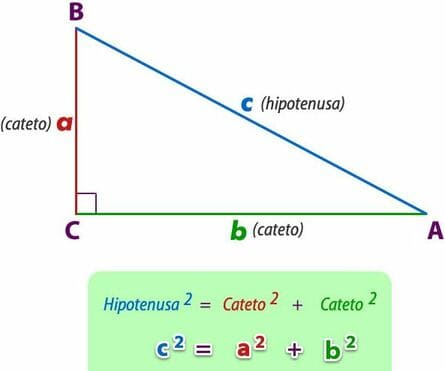
\includegraphics[width=0.3\textwidth]{book/Spanish/03_Conditionals_if_elif_else/images/ejemplo-del-teorema-de-pitagoras.jpeg}

La distancia al origen del punto (x, y) es la raíz cuadrada de la suma de los cuadrados de sus coordenadas. Para calcular la raíz cuadrada en Python podemos usar la función: math.sqrt():\\

\begin{Verbatim}[frame=single]
>>> import math
>>> math.sqrt(25)
5.0
>>> 
\end{Verbatim}

Puedes ejecutar los siguientes tests:\\

\begin{Verbatim}[frame=single, label={\em example test execution of the program}]
>>> %Run 
  coordenado x del 1er punto en el plano: 2.5
  coordenado y del 1er punto en el plano: 3.03
  coordenado x del 2do punto en el plano: 6
  coordenado y del 2do punto en el plano: 7.4
  punto (2.5,3.0) esta el mas proximo al origen
>>> %Run 
  coordenado x del 1er punto en el plano: 5
  coordenado y del 1er punto en el plano: 9
  coordenado x del 2do punto en el plano: -2
  coordenado y del 2do punto en el plano: 0
  punto (-2.0,0.0) esta el mas proximo al origen
>>> %Run 
  coordenado x del 1er punto en el plano: 0
  coordenado y del 1er punto en el plano: 0
  coordenado x del 2do punto en el plano: 0
  coordenado y del 2do punto en el plano: 0
  distancia al origen es igual para ambos puntos
>>> %Run 
  coordenado x del 1er punto en el plano: 1
  coordenado y del 1er punto en el plano: 3
  coordenado x del 2do punto en el plano: -8
  coordenado y del 2do punto en el plano: 1
  punto (1.0,3.0) esta el mas proximo al origen
\end{Verbatim}
 
Es estos 3 ejecuciones estamos haciendo tests para:

\begin{itemize}
    \item primer punto (cuadrante I), segundo punto (cuadrante I)
    \item primer punto (cuadrante I), segundo punto (cuadrante II)
    \item primer punto (cuadrante I), segundo punto (cuadrante IV)
    \item ambos puntos son el origen
\end{itemize}

 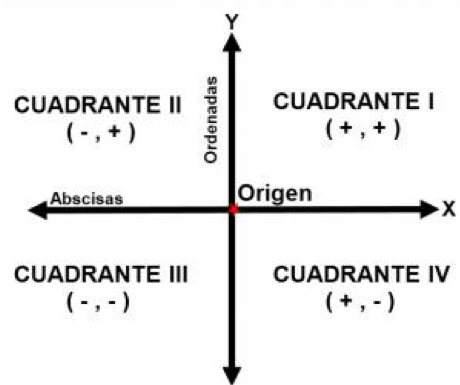
\includegraphics[]{images/cuadrant.png}

Si queremos probar todas las combinaciones de los cuadrantes. ¿que otros tests tenemos que correr?
\end{ejercicio}

\begin{ejercicio}(difícil) Escribe un programa en Python que pide al usuario cuatro valores enteros y mostrarlos por pantalla de mayor a menor. Cuando empieces a pensar en la solución te darás cuanta que no es tan fácil como parece a primera vista.
\end{ejercicio}

\begin{ejercicio}Adapta todos los programas de los ejercicios anteriores que pueden lanzar un \pythoninline{ValueError} cuando el usuario no teclea un valor el tipo adecuado. Utiliza la construcción de \pythoninline{try-except}. 

Por ejemplo para el ejercicio \ref{coords}:\\

\begin{Verbatim}[frame=single, label={\em ejemplos y posibles tests de ejecución}]
>>> %Run 
  coordenado x del 1er punto en el plano: r
  No has introducido el tipo correcto. Se necesita: floats
\end{Verbatim}
\end{ejercicio}



